\documentclass[a4paper, 10pt]{article}[5.10.2011]
%% packages
\usepackage[left=2cm, text={17cm, 24cm}, top=3cm]{geometry} % rozmery stránky
\usepackage[czech]{babel}
\usepackage[utf8]{inputenc}
\usepackage[IL2]{fontenc}
\usepackage{colortbl}
\usepackage{graphicx}
\newcommand{\czuv}[1]{\quotedblbase#1\textquotedblleft}
\definecolor{gray}{rgb}{0.4,0.4,0.4}
% =======================================================================
% balíček "hyperref" vytváří klikací odkazy v pdf, pokud tedy použijeme pdflatex
% problém je, že balíček hyperref musí být uveden jako poslední, takže nemůže
% být v šabloně
\usepackage{color}
\usepackage[unicode,colorlinks,hyperindex,plainpages=false]{hyperref}
\definecolor{links}{rgb}{0.4,0.5,0}
\definecolor{anchors}{rgb}{1,0,0}
\def\AnchorColor{anchors}
\def\LinkColor{links}
\def\pdfBorderAttrs{/Border [0 0 0] } % bez okrajů kolem odkazů
\pdfcompresslevel=9




\title{Paralelní a distribuované algoritmy\,--\,dokumentace\\ Projekt 1 : Pipeline merge sort}
\author{Bc. Marek Kidon}
\date{\today}
\begin{document}
\maketitle
\noindent Dokumentace k 1.projektu do předmětu Paralelní a distribuované algoritmy (PRL). V dokumentu je rozebráno zadaní, popis řešení, analýza algoritmu PMS, časová složitost, naměřené hodnoty času potřebného pro seřazení v závislosti na počtu prvků a komunikace mezi \textit{sortery}. Časová složitost je zobrazena formou grafu a komunikace je zobrazena za použití \textit{Message Sequence Chart} diagramu.
\section{Zadání projektu}
Pomocí knihovny Open MPI implementujte v jazyce C/C++ algoritmus \textbf{Pipeline merge sort}.
\subsection*{Vstup}
Soubor \textit{numbers} obsahující čísla velikosti 1 byte, která jdou bez mezery za sebou.
\subsection*{Výstup}
Výstup na stdout se skládá ze dvou částí: 
\begin{enumerate}
\item Jednotlivé načtené hodnoty v jednom řádku oddělené mezerou (vypsat po načtení prvním procesorem).
\item Jednotlivé seřazené hodnoty oddělené novým řádkem (od nejmenšího po největší).
\end{enumerate}
\subsection*{Postup řešení}
Vytvořte testovací skript test, který bude řídit testování. Tento skript bude mít tyto vlastnosti:
\begin{enumerate}
	\item Bude pojmenován \textit{test} nebo \textit{test.sh}.
	\item Bude přijímat 1 parametr a to \textit{pocet\_hodnot}.
\end{enumerate}

Skript vytvoří podle velikosti parametru \textit{pocet\_hodnot} soubor \textit{numbers} s náhodnými čísly a následně spustí program s počtem procesorů \textit{log\_2(pocet\_hodnot)+1}. Skript nakonec smaže vytvořenou binárku a soubor \textit{numbers}. 

\section{Analýza algoritmu}
Algoritmus řadí za pomocí \textit{lineárního pole procesorů}. Data lineárně prochází polem procesorů, každý procesor $P_{i}$ sloučí 2 seřazené posloupnosti délky $2^{i-2}$ do jedné posloupnosti délky $2^{i-1}$. Všechny procesory beží paralelně. Jednotlivé procesory jsou spojeny frontami, 2 vstupní a 2 výstupní. Výjimku tvoří první a poslední procesor, kde první má jednu vstupní frontu a poslední jen jednu výstupní. 
\begin{itemize}
\item Každý procesor začíná, když má v první frontě seřezenou posloupnost alespoň délky $2^{i-2}$ a v druhé alespoň 1 prvek.
\item $P_{i}$ začne svou činnost v cyklu $$1 + \sum^{i-2}_{j=0} 2^j + 1 = 2^{i-1} + i -1$$.
\item Algoritmus skončí za $(n-1) + 2^{i-1} + i - 1$ cyklů. 
\end{itemize}

	Pro samotné sloučení 2 posloupností stačí operace porovnání. Není třeba žádného seřazování, neboť vstupní posloupnosti již seřazené jsou. Stačí tedy porovnávat vždy jen ty prvky, které se nachází ve frontě na prvním místě. A do výstupní fronty zařadit ten, jež je větší (menší) v případě, že řadíme sestupně (vzestupně). Volba výstupní fronty probíha dle počtu již odeslaných čisel, a to za pomocí následující operace zbytkových tříd : $(counter / base) \% 2$, kde $counter$ je počet již odeslaných prvků a $base$ je základ dle vzorce $2^{i-2}$.

\section{Složitost a Optimálnost}
\textbf{Časová složitost algoritmu}:\textit{t(n)=O(n)}\\
Algoritmus je \textbf{optimální}:\textit{$c(n)$}=\textit{$t(n)$}$.$\textit{$p(n)$}=\textit{$O(n.\log n)$}

\section{Naměřené hodnoty}
Měření bylo provedeno za použití knihovny \textit{chrono}, a měřil se čas potřebný k seřazení dané posloupnosti měřeno od začátku práce prvního \textit{sorteru} po dokončení práce posledního. Výsledky jsou dané v časových jednotkách, mohou se tedy při ruznách bězích lišit, kvůli přepínání kontextu operačního systému. Celý test byl proveden při stabilním zatížení stroje a pokusy nad jednolivými vstupními sekvencemi o stejné délce byly provedeny několikrát a aritmeticky zprůměrovány. O přes výše uvedenou nepřesnost, závislost mezi jednotlivými hodnotami v tabulce odpovídá a na výslednou křivku nemá vliv. \\
Pro měření mělo 2 specifika odchylující se od zadání. Pro generovnání byl namísto zdroje \textit{/dev/random} použit \textit{/dev/urandom}. Veškerý výstup na stdout byl přesměrován do \textit{/dev/null}.

\begin{table}[ht]
\begin{center}
\begin{tabular}{ l | c c c c c c c c c c }
%\rowcolor[gray]{0.9}
\hline
\textbf{počet prvků} & 2 & 4 & 8 & 16 & 32 & 64 & 128 & 256 & 512 \\
\textbf{čas[s]} & 0.00126 & 0.00213 & 0.00231 & 0.00377 & 0.00574 & 0.01076 & 0.01923 & 0.03917 & 0.10286 \\ \hline
\end{tabular}
\end{center}

\begin{center}
\begin{tabular}{ l | c c c c c c}
\hline
\textbf{počet prvků} & 1024 & 2048 & 4096 & 8192 & 16384 & 32768  \\
\textbf{čas[s]} & 0.10987 & 0.44353 & 0.83116 & 1.54915 & 3.27791 & 3.67929 \\ \hline
\end{tabular}
\caption{Přehled naměřených časů v závislosti na počtu prvků.}
\label{tab1}
\end{center}
\end{table}

Na obrázku \ref{pic1} je graficky znázorněn vztah mezi počtem prvků a časem potřebným k jejich seřazení.
\begin{figure}[ht]
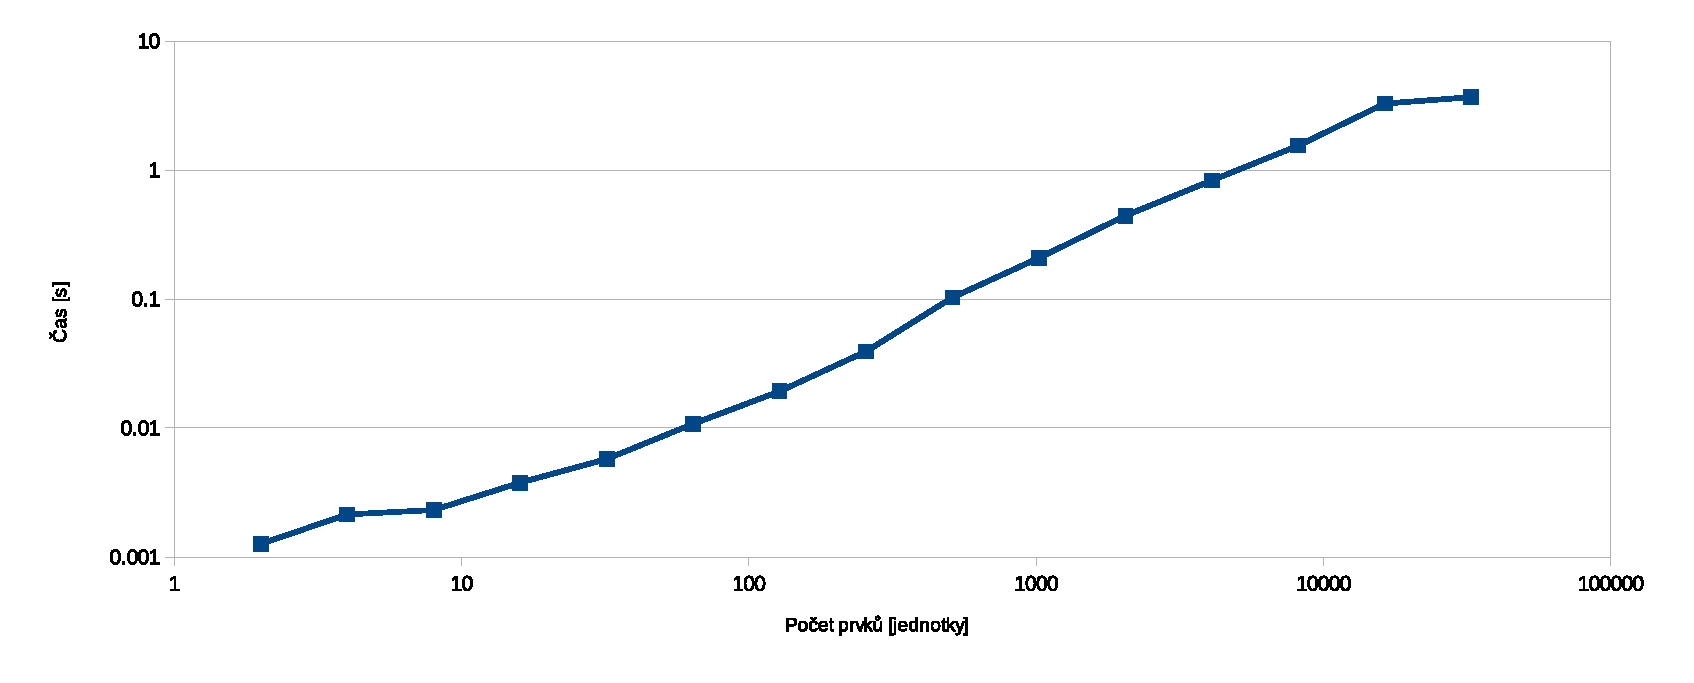
\includegraphics[scale=.6]{1.eps}
\caption{Závislost počtu prvků na časem nutném k jejich seřazení.}
\label{pic1}
\end{figure}

%Vzhledem k exponenciálnímu nárůstu počtu hodnot, bylo pro zobrazení v grafu použito logaritmické měřítko na obou osách.%% což vrátí složitost zpět na lineární křivku.

\section{Komunikace mezi procesory}
Procesory mezi sebou používají velmi jednoduchý komunikační protokol. Aby se předešlo komplikovaným scénářům, Každý procesor komunikuje pouse se svým následníkem, nikoli se svým předchůdcem. Je všal nutné, aby při zasílání zprávy,
procesor vždy vědel, do které fronty následníka má číslo umístit. Na počátku první procesor po zpracování vstupu, rozešle všem procesorům informaci o celkovém počtu prvků. Ten je použit jako ukončovací podmínka. Poté začína samotné řazení. Prvky jsou vybírány z front pomocí operace $<=$ v případě, že jsou obě fronty neprázdné nebo je prvek vybrán bez porovnání, v případě, že opačná fronta je prázdná.

\begin{figure}[ht]
\centering
\small\begin{verbatim}
          
          +-------------+      +-------------+      +-------------+      +-------------+
          + 1. Procesor +      + 2. Procesor +      + 3. Procesor +      + 4. Procesor +
          +-------------+      +-------------+      +-------------+      +-------------+
                 |                    |                    |                    |
                 | BCAST:celkem cisel |                    |                    |
                 |------------------->| BCAST:celkem cisel |                    |
                 |--------------------|------------------->| BCAST:celkem cisel |
                 |--------------------|--------------------|------------------->|
                 |                    |                    |                    |
                 | MSG:1/1 do f. 1    |                    |                    |
                 |------------------->|                    |                    |
                 | MSG:1/1 do f. 2    | MSG:1/2 do f. 1    |                    |
                 |------------------->|------------------->|                    |
                 | MSG:1/1 do f. 1    | MSG:2/2 do f. 1    |                    |
                 |------------------->|------------------->|                    |
                 | MSG:1/1 do f. 2    | MSG:1/2 do f. 2    |                    |
                 |------------------->|------------------->| MSG:1/4 do f. 1    |
                 | MSG:1/1 do f. 1    | MSG:2/2 do f. 2    |------------------->|
                 |------------------->|------------------->| MSG:2/4 do f. 1    |
                 | MSG:1/1 do f. 2    | MSG:1/2 do f. 1    |------------------->|
                 |------------------->|------------------->| MSG:1/4 do f. 1    |
                 | MSG:1/1 do f. 1    | MSG:2/2 do f. 1    |------------------->|
                 |------------------->|------------------->| MSG:2/4 do f. 1    |
                 | MSG:1/1 do f. 2    | MSG:1/2 do f. 2    |------------------->|
                 |------------------->|------------------->| MSG:1/4 do f. 2    |
                 |                    | MSG:2/2 do f. 2    |------------------->|
                 |                    |------------------->| MSG:2/4 do f. 2    |
                 |                    |                    |------------------->|
                 |                    |                    | MSG:1/4 do f. 2    |
                 |                    |                    |------------------->|
                 |                    |                    | MSG:2/4 do f. 2    |
                 |                    |                    |------------------->|
                 |                    |                    |                    |
          
          
\end{verbatim}
\caption{Ukázka zasílání zpráv mezi prvními čtyřmi procesory. Diagram by mohl pokračovat pro další procesory analogicky.}
\label{pic}
\end{figure}

\normalsize
\end{document}


